\documentclass[a4paper,fleqn]{article}
\usepackage{amsmath}
\usepackage{amsfonts}
\usepackage{eqparbox}
\usepackage{mathtools}
\usepackage{hyperref}
\usepackage{arcs}
\usepackage{graphicx}
\usepackage[margin=0.6in]{geometry}

\graphicspath{ {.} }

\newcommand{\neweq}[2]{
        #1 = 
        \begin{pmatrix*}[r]
            #2
        \end{pmatrix*}
}

\newcommand{\newvec}[1]{
    \begin{pmatrix*}[r]
        #1
    \end{pmatrix*}
}

\newcommand{\newdet}[1]{
    \begin{vmatrix}
        #1
    \end{vmatrix}
}

\begin{document}
    \Large{\textbf{Q1:}}
    % \begin{equation*}
    % \neweq{\mathbf{x}}{1\\2\\3\\4\\5i}
    % \hspace{2cm}
    % \neweq{\mathbf{y}}{1\\4\\-2\\0\\1}
    % \end{equation*}

    \begin{enumerate}
    \item \(
    \neweq{\mathbf{x} + \mathbf{y}}{2\\6\\1\\4\\1+5i}
    \) 

    \item \(
    \langle\mathbf{x, y}\rangle = \mathbf{x^\dagger*y} 
    = \newvec{1 & 2 & 3 & 4 & -5i}*\newvec{1\\4\\-2\\0\\1} \\
    = 1\times1+2\times4-3\times2+0-1\times5i
    = 3-5i
    \)

    \item \(
    \mathbf{y^\dagger x} 
    = \newvec{1&4&-2&0&1}*\newvec{1\\2\\3\\4\\5i}
    = 1\times1+4\times2-2\times3+0+5i
    = 3+5i
    \)

    \item \(
    \mathbf{x\circ y}
    =\newvec{1\times1\\2\times4\\3\times-2\\4\times0\\5i\times1}
    =\newvec{1\\8\\-6\\0\\5i}
    \)

    \item \(
    \mathbf{xy^\dagger} 
    =\newvec{1\\2\\3\\4\\5i}*\newvec{1&4&-2&0&1}
    =\newvec{1*\newvec{1&4&-2&0&1}\\2*\newvec{1&4&-2&0&1}\\3*\newvec{1&4&-2&0&1}\\4*\newvec{1&4&-2&0&1}\\5i*\newvec{1&4&-2&0&1}}
    =\newvec{1&4&-2&0&1\\2&8&-4&0&2\\3&12&-6&0&3\\4&16&-8&0&4\\5i&20i&-10i&0&5i}
    \)

    \item Because $\mathbf{xy^\dagger}$ is the linear combination of $\mathbf{y^\dagger}$ and $\mathbf{y^\dagger}$ is a real matrix, so $\mathbf{y^\dagger=y^T}$ and $Rank(xy^\dagger)=Rank(y^\dagger)=Rank(y^T)=Rank(y)=1$
    
    \end{enumerate}

    \newpage
    \Large{\textbf{Q2:}}
    \begin{enumerate}
        \item 
        $\|\mathbf{x}\|_2 = (\sum\limits_{i,j=1}^n |x_{i,j}|)^\frac{1}{2} = \sqrt{1^2+2^2+3^2+4^2+|5i^2|} = \sqrt{55}=7.4162$

        \item 
        $\|\mathbf{xy^\dagger}\|=\sqrt{1210}=34.7851$

        In MATLAB, use $norm(x, 2)$
    \end{enumerate}

    \newpage 
    \Large{\textbf{Q3}}
    \begin{enumerate}
        \item For $\mathbf{A}$, 
        
        $det{(\mathbf{A})} = 1*\newdet{1&2&4\\2&1&3\\4&3&1}-(-1)*\newdet{-1&2&4\\0&1&3\\i&3&1}+0*\newdet{-1&1&4\\0&2&3\\i&4&1}-(-i)*\newdet{-1&1&2\\0&2&1\\i&4&3}\\
        =20+8+2i+3-2i
        =31 > 0$

        \vspace{0.5cm}
        Because $det(\mathbf{A})>0$, $\mathbf{A}$ is the full-rank matrix. $Rank(\mathbf{A}) = 4$
        
        For any matrix $\mathbf{x}$, $Rank(\mathbf{x})+nullity(\mathbf{x})=n$, so the dimension of $\mathbf{x}$'s null space is: \\
        $nullity(\mathbf{A})=4-Rank(\mathbf{A})=0$
        
        \item For $\mathbf{B}$, \\
        $\mathbf{B}=\newvec{1&4&3\\2&3&1\\3&2&-1} \stackrel{rref}{=}\newvec{1&4&3\\0&-5&-5\\0&0&0}$ 

        $Rank(\mathbf{B}) = 2$ 

        $nullity(\mathbf{B}) = 3 - 2 =1$

        \item For $\mathbf{C}$, \\
        $\mathbf{C} = \newvec{2&3\\-3&0.5} \stackrel{rref}{=}\newvec{2&3\\0&5}$

        \vspace{0.5cm}
        $Rank(\mathbf{C})=2$

        \vspace{0.5cm}
        $nullity(\mathbf{C}) = 2 - 2 =0$

        \vspace{0.5cm}
        $det(\mathbf{C})=\newdet{2&3\\-3&0.5}=1-(-9)=10$

        \vspace{0.5cm}
        $\mathbf{C}^{-1}=\frac{1}{det({\mathbf{C}})}\newvec{0.5&-3\\3&2}=\newvec{0.05&-0.3\\0.3&0.2}$

        \vspace{0.5cm}
        $\mathbf{C}+\mathbf{C}^T = \newvec{2&3\\-3&0.5}+\newvec{2&-3\\3&0.5}=\newvec{4&0\\0&1}$

        eigenvalues of $\mathbf{C}+\mathbf{C}^T$ is $\lambda_1=4, \lambda_2=1$

        \vspace{0.5cm}
        $\mathbf{C}-\mathbf{C}^T = \newvec{2&3\\-3&0.5}-\newvec{2&-3\\3&0.5}=\newvec{0&6\\-6&0}$

        eigenvalues of $\mathbf{C}-\mathbf{C}^T$ is $\lambda_1=6i, \lambda_2=-6i$
    \end{enumerate}

    \newpage
    \Large{\textbf{Q4:}}
    \begin{enumerate}
        \item First, calculate the inverse of $\mathbf{A}\mathbf{A}^T$:
        
        $\mathbf{A}\mathbf{A}^T=\newvec{1&0&3\\2&-1&-2}*\newvec{1&2\\0&-1\\3&-2}=\newvec{10&-4\\-4&9} 
        \Longrightarrow 
        (\mathbf{A}\mathbf{A}^T)^{-1}=inv(\mathbf{A}\mathbf{A})=\frac{1}{74}\newvec{9&4\\4&10}=\newvec{0.1216&0.0541\\0.0541&0.1351}$\\
        Then $\mathbf{A}^T(\mathbf{A}\mathbf{A}^T)^{-1}=\newvec{1&2\\0&-1\\3&-2}*\newvec{9&4\\4&10}=\newvec{0.2297&0.3243\\-0.0541&-0.1351\\0.2568&-0.1081}$

        \item $\mathbf{AA^+}=\newvec{1&0&3\\2&-1&-2}*\newvec{0.2297&0.3243\\-0.0541&-0.1351\\0.2568&-0.1081}=I_2$. So its dimension is 2. 
        
        \item $\mathbf{A^+A}=\newvec{0.2297&0.3243\\-0.0541&-0.1351\\0.2568&-0.1081}*\newvec{1&0&3\\2&-1&-2}=\newvec{0.8784&-0.3243&0.0405\\-0.3243&0.1351&0.1081\\0.0405&0.1081&0.9865} \\
        \stackrel{rref}{=} \newvec{1&0\\0&1\\0&0}$. Its dimension is $3\times 2$. 
    \end{enumerate}

    \newpage
    \Large{\textbf{Q5:}}

    \noindent $\mathbf{ABC(ABC)^T=I} \Longrightarrow \mathbf{ABC}=\mathbf{(.)}_{M\times Q}$ is semi-orthogonal if $M < Q$ or orthogonal if $M=Q$. So when $\mathbf{A, B, C}$ are semi-orthogonal so that $\mathbf{AA^T=I_M; BB^T=I_N;}$ \\ $\mathbf{CC^T=I_P}$ if $M < N, N < P, P < Q$ or orthogonal so that $\mathbf{AA^T=BB^T=CC^T=I_M}$ if $M=N=P=Q$, then:  
    
    \vspace{0.5cm}
    \noindent $\mathbf{ABC(ABC)^T}=\mathbf{AB(CC^T)B^TA^T}=\mathbf{A(BI_PB^T)A^T}=\mathbf{AI_NA^T}=\mathbf{I_M}$ \\
    So its $dim(.) = M$

    \newpage
    \Large{\textbf{Q6:}}

    $\mathbf{AA^\dagger}=\frac{1}{\sqrt{2}}\newvec{1+i&1-i&1+i\\1-i&1+i&1-i\\1+i&1-i&1+i}*\frac{1}{\sqrt{2}}\newvec{1-i&1+i&1-i\\1+i&1-i&1+i\\1-i&1+i&1-i}=\newvec{3&0&3\\0&2&0\\3&0&3}$

    $\mathbf{BB^T}=\mathbf{B*B}=\newvec{1&0&0&0\\0&1&0&0\\0&0&1&0\\0&0&0&1}$

    $\mathbf{CC^T}=\frac{1}{3}\newvec{1&2&2\\-2&-1&2\\2&-2&1}*\frac{1}{3}\newvec{1&-2&2\\2&-1&-2\\2&2&1}=\newvec{1&0&0\\0&1&0\\0&0&1}$

    \noindent Because $\mathbf{B}$ is a symmetric matrix, $\mathbf{B}=\mathbf{B^T}\Longrightarrow\mathbf{BB^T}=\mathbf{BB}=\mathbf{B^2}$ \\
    $\mathbf{A}$ is not a Hermitian matrix, not conjugate symmetric, therefore $\mathbf{AA^\dagger \neq A^2}$. \\
    $\mathbf{C}$ is not a symmetric matrix, therefore $\mathbf{CC^T\neq C^2}$.

    \newpage
    \Large{\textbf{Q7:}}

    $\frac{\partial f(\mathbf{x})}{\partial \mathbf{x}} = e^{-\frac{1}{2}\mathbf{x^T K^{-1} x}}
    *(-\frac{1}{2}\mathbf{x^T K^{-1} x})^{'}=e^{-\frac{1}{2}\mathbf{x^T K^{-1} x}}*-\frac{1}{2}(2\mathbf{K^{-1}x})
    =e^{-\frac{1}{2}\mathbf{x^T K^{-1} x}}\mathbf{K^{-1}x} $
    
    \vspace{1cm}
    As for its dimension, $\mathbf{K^{-1}x}=(.)_{N\times 1}$ and $\mathbf{x^T K^{-1} x}=(.)_{1\times 1} \\ 
    \indent\Longrightarrow dim(\frac{\partial f(\mathbf{x})}{\partial \mathbf{x}})=dim(\mathbf{K^{-1}x})=N\times 1$

    \newpage
    \Large{\textbf{Q8:}}

    \noindent For $\mathbf{A}$, $det(\mathbf{A}-\lambda I)=0 \Longrightarrow eig(A)$ in MATLAB: Then its eignevalues are: \\ 
    $\lambda_1=11.0632, \lambda_2=2.922, \lambda_3=-0.9791+0.3559i, \lambda_4=-0.9791-0.3559i$\\
    $\mathbf{A}$'s corresponding diagonal matrix $\mathbf{D}$ is: \\
    $\mathbf{D} = \newvec{11.0632\\&2.922\\&&-0.9791+0.3559i\\&&&-0.9791-0.3559i}$\\
    The corresponding nonsingular matrix $\mathbf{\Lambda}$ (via $\mathbf{[\Lambda, D]=eig(A)}$): \\
    $\mathbf{\Lambda}=\newvec{-0.5140&0.5688&0.5378 + 0.0107i&0.5378 - 0.0107i\\-0.3665& -0.7124&  0.4333 - 0.1353i&   0.4333 + 0.1353i\\-0.5291&  0.2034&  -0.6356& -0.6356&\\-0.5671& -0.3573&  -0.2862 + 0.1366i & -0.2862 - 0.1366i}$\\
    so that $\mathbf{\Lambda D\Lambda^{-1}=A}$

    \vspace{0.5cm}
    \noindent For $\mathbf{B}$, same operation as $\mathbf{A}$, then its eigenvalues are:\\
    $\lambda_1=-2.1487,\lambda_2=0.0770,\lambda_3=4.3554,\lambda_4=9.7164$ \\
    $\mathbf{B}$'s diagonal matrix $\mathbf{D}$ is: \\
    $\mathbf{D}=\newvec{-2.1487\\&0.0770\\&&4.3554\\&&&9.7164}$ \\
    and corresponding nonsingular matrix $\mathbf{\Lambda} = \newvec{0.2041&0.6932&-0.3318&0.6064\\0.6640&-0.2284&0.6081&0.3704\\-0.1256&-0.6754&-0.4595&0.5630\\-0.7083&0.1054&0.5559&0.4221}$\\
    \noindent\rule{\textwidth}{0.4pt}
    \noindent Before calculating the eigenvalues, its easy to predict $\mathbf{B}$ has real eignevalues, since its a \textbf{real symmetric matrix}. \\
    \textbf{Proof:} $\mathbf{B}$ is a real symmetric matrix, so $\mathbf{B}=\mathbf{B^T}=\mathbf{\bar{B}}$. Assume $\lambda$ is a complex eigenvalue and $\mathbf{x}$ is the complex eigenvector of $\mathbf{B}$, and $\bar{\lambda}$ and $\mathbf{\bar{x}}$ are the corresponding conjugate complex and conjugate vector, then we have \\
    $\mathbf{B\bar{x}=\bar{B}\bar{x}=(\bar{Bx})=(\bar{\lambda x})=\bar{\lambda}\bar{x}}$ 
    \begin{equation} \label{eqn:1}
        \mathbf{\bar{x}^TBx=\bar{x}^T(Bx)=\bar{x}^T\lambda x=\lambda \bar{x}^T x}
    \end{equation}
    \vspace{-1cm}
    \begin{equation} \label{eqn:2}
        \mathbf{\bar{x}^TBx=(x^TB^T)x=(B\bar{x})^Tx=(\bar{\lambda} \bar{x})^T x=\bar{\lambda} \bar{x}^T x}
    \end{equation}
    Let (~\ref{eqn:1})-(~\ref{eqn:2}), we get $(\lambda-\bar{\lambda})\mathbf{\bar{x}^Tx}=0$. Since $\mathbf{x}$ is not $0$, $\lambda = \bar{\lambda}$. Therefore, $\lambda$ is real. \\
    \noindent\rule{\textwidth}{0.4pt}
    \noindent As for $A$, the characteristic polynomials format of its eigenvalues is $det(\mathbf{A-\lambda E}) = x^4-12x^3+6x^2+48x+35=0$. According to \href{https://en.wikipedia.org/wiki/Descartes%27_rule_of_signs}{\textbf{Descartes' rule of signs}}, we could get the number of positive and negative real roots in a polynomial. Let $f(x)=\underrightarrow{x^4-12}\underrightarrow{x^3+6}x^2+48x+35$ and $f(-x)=x^4+12x^3+6\underrightarrow{x^2-48}\underrightarrow{x+35}$, there are both 2 sign changes, indicating 2 or 0 positive roots and 2 or 0 negative roots. Therefore, $number of complex roots = n-p-q \ge 0$, where $n$ is the degree of polynomials (here is 4), and $p$ and $q$ are the number of positive and negataive roots respectively. It's high likely that $\mathbf{A}$ has complex roots. 

    \newpage
    \Large{\textbf{Q9:}}

    $\mathbf{A}=\newvec{1 &1 &2 &2\\ 1 &3 &3 &2\\ 3 &1 &3 &2\\ 2 &6 &6 &4}\stackrel{rref}{=}\newvec{1&0&0&-1\\0&1&0&-1\\0&0&1&2\\0&0&0&0}$\\
    After adding the noise $\mathbf{N}=\newvec{-0.0065&-0.0085&-0.0020&-0.0151\\0.0118&-0.0057&0.0059&0.0088\\-0.0076&-0.0056&-0.0085&-0.0024\\-0.0111&0.0018&0.0080&0.0017}$, the bottom row of $\mathbf{A}$ would be no longer 0. Since the noise row is less likely to be a linear combination of previous 3 rows, making the noised matrix $\mathbf{A}+N$ full rank, which means the inverse matrix exists.  

    \noindent However, because the noise only adds trivial value to original matrix, its eigenvalues changes little. The eigenvalues of $\mathbf{A}$ and eigenvalues of $\mathbf{A+N}$ are:\\
    $\mathbf{vec_{\lambda 1}}=\newvec{10.5625\\0.2188+0.5752i\\0.2188-0.5752i\\0.0000}$, $\mathbf{vec_{\lambda 2}}=\newvec{10.5552\\0.1969 + 0.5579i\\0.1969 - 0.5579i \\0.0320}$ \\
    $\Delta\mathbf{vec_\lambda}=\mathbf{vec_{\lambda 1}}-\mathbf{vec_{\lambda 2}}=\newvec{0.0073\\0.0219 + 0.0173i\\0.0219 - 0.0173i\\-0.0320}$ and $mean(\Delta\mathbf{vec_\lambda})=0.0048$ \\
    We can see that the eigenvalues doesn't change a lot when $\alpha=0.01$. If the $\alpha$ increase, the eigenvalues also change more and vice versa, as the following image shows.
    
    \begin{figure}[!ht]
        \centering
        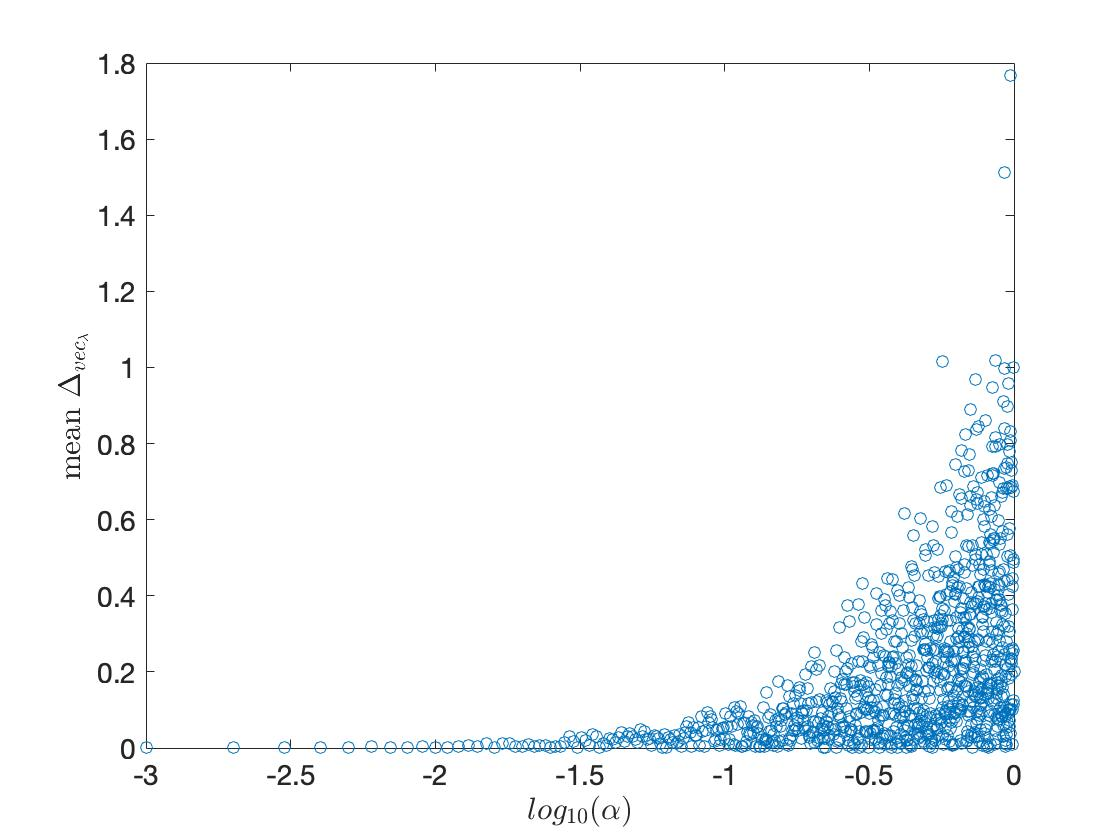
\includegraphics[width=0.7\textwidth]{diff_alpha.jpg}
        \caption{$\mathbf{A}$'s eigenvalues change under different noise amplitude $\alpha$. Not axis $y$ is the $mean(\Delta_{\mathbf{vec_\lambda}})$; axis $x$ is the $log_{10}$ value of $\alpha$. We tested $\alpha$ from 0.001 to 1 with 0.001 as the stride.}
    \end{figure}

\end{document}